\documentclass[tikz,border=8pt]{standalone}
\usepackage{amsmath,amssymb}
\usetikzlibrary{arrows.meta,calc}

\begin{document}
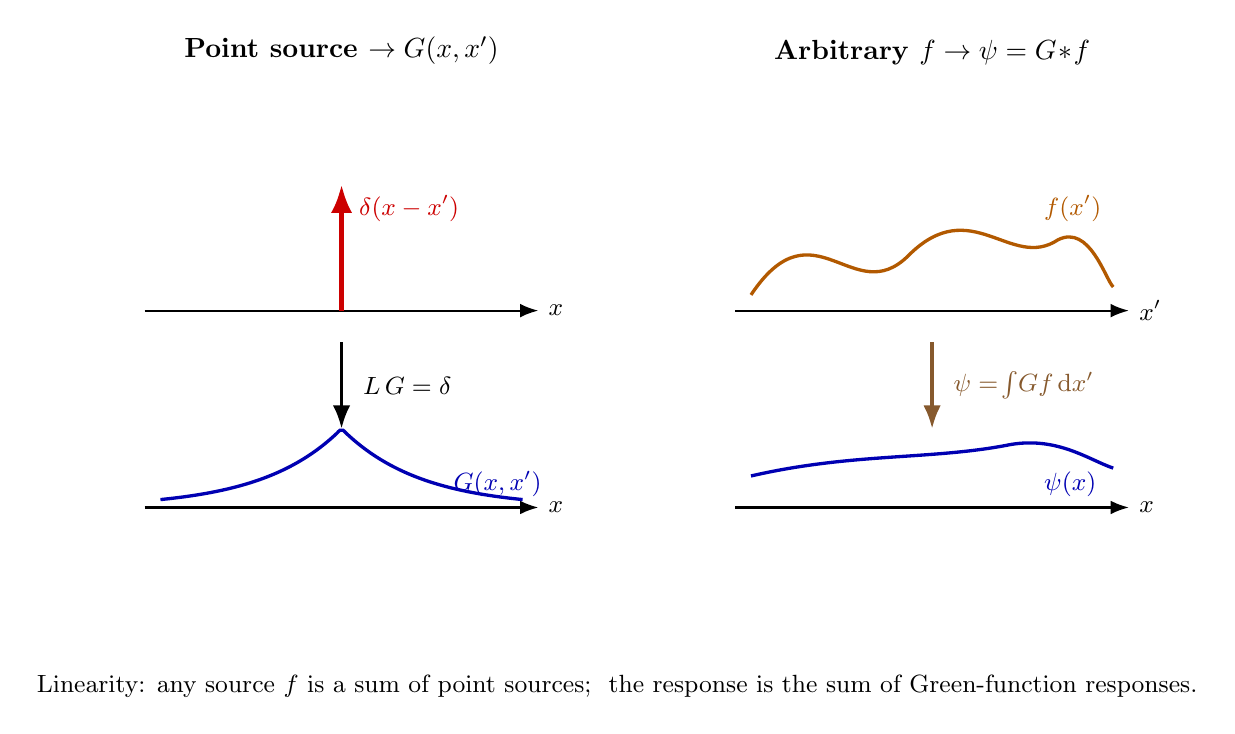
\begin{tikzpicture}[>=Latex]

  % LEFT: point source -> Green's function
  \begin{scope}[xshift=0cm]
    \node[font=\bfseries, anchor=south] at (0, 3.0) {Point source $\to G(x,x')$};

    \draw[->, thick] (-2.5, 0) -- (2.5, 0) node[right, font=\small]{$x$};
    \draw[->, ultra thick, red!80!black] (0, 0) -- (0, 1.6);
    \node[font=\small, red!80!black, anchor=west] at (0.1, 1.3) {$\delta(x-x')$};

    \begin{scope}[yshift=-2.5cm]
      \draw[->, thick] (-2.5, 0) -- (2.5, 0) node[right, font=\small]{$x$};
      \draw[blue!70!black, very thick, smooth, samples=120, domain=-2.3:2.3]
        plot(\x, {1.0*exp(-abs(\x))});
      \node[font=\small, blue!70!black, anchor=west] at (1.3, 0.3) {$G(x,x')$};
    \end{scope}

    \draw[->, very thick] (0, -0.4) -- (0, -1.5);
    \node[font=\small, anchor=west] at (0.15, -0.95) {$L\,G=\delta$};
  \end{scope}

  % RIGHT: arbitrary source -> response
  \begin{scope}[xshift=7.5cm]
    \node[font=\bfseries, anchor=south] at (0, 3.0) {Arbitrary $f \to \psi=G\!*\!f$};

    \draw[->, thick] (-2.5, 0) -- (2.5, 0) node[right, font=\small]{$x'$};
    \draw[orange!70!black, very thick, smooth]
      (-2.3, 0.2) .. controls (-1.5, 1.4) and (-1.0, 0.0) .. (-0.3, 0.7)
       .. controls (0.5, 1.5) and (1.0, 0.5) .. (1.6, 0.9)
       .. controls (2.0, 1.1) and (2.2, 0.4) .. (2.3, 0.3);
    \node[font=\small, orange!70!black, anchor=west] at (1.3, 1.3) {$f(x')$};

    \begin{scope}[yshift=-2.5cm]
      \draw[->, thick] (-2.5, 0) -- (2.5, 0) node[right, font=\small]{$x$};
      \draw[blue!70!black, very thick, smooth]
        (-2.3, 0.4) .. controls (-1.0, 0.7) and (0.0, 0.6) .. (1.0, 0.8)
         .. controls (1.6, 0.9) and (2.0, 0.6) .. (2.3, 0.5);
      \node[font=\small, blue!70!black, anchor=west] at (1.3, 0.3) {$\psi(x)$};
    \end{scope}

    \draw[->, very thick, brown!70!black] (0, -0.4) -- (0, -1.5);
    \node[font=\small, anchor=west, brown!70!black] at (0.15, -0.95) {$\psi=\!\int\! G f\,\mathrm dx'$};
  \end{scope}

  % bottom unifying
  \node[font=\small, anchor=north, align=center] at (3.5, -4.5)
    {Linearity: any source $f$ is a sum of point sources;\ \ the response is the sum of Green-function responses.};
\end{tikzpicture}
\end{document}
